\documentclass[12pt,twoside]{article}
\usepackage{amsmath, amssymb}
\usepackage{amsmath}
\usepackage[active]{srcltx}
\usepackage{amssymb}
\usepackage{amscd}
\usepackage{makeidx}
\usepackage{float}
\usepackage{amsthm}
\usepackage{algpseudocode}
\usepackage{algorithm}
\usepackage{graphicx}
\usepackage[spanish, es-tabla]{babel}
\usepackage{multirow}
\usepackage{cite}
\renewcommand{\baselinestretch}{1}
\graphicspath{{images/}}
\setcounter{page}{1}
\setlength{\textheight}{21.6cm}
\setlength{\textwidth}{14cm}
\setlength{\oddsidemargin}{1cm}
\setlength{\evensidemargin}{1cm}
\pagestyle{myheadings}
\thispagestyle{empty}
\markboth{\small{Pr\'actica 10. Alan, Josu\'e}}{\small{.}}
\date{}
\begin{document}
\centerline{\bf An\'alisis de Algoritmos, Sem: 2020-1, 3CV2, Pr\'actica 10, 20 de noviembre}
\centerline{}
\centerline{}
\begin{center}
\Large{\textsc{Pr\'actica 10: Estrategia Greedy.}}
\end{center}
\centerline{\bf{Alan Romero Lucero, Josu\'e David Hern\'andez Ram\'irez}}
\centerline{}
\centerline{Escuela Superior de C\'omputo}
\centerline{Instituto Polit\'ecnico Nacional, M\'exico}
\centerline{$alanrl.escom@gmail.com, josuehernandezr082@gmail.com$}
\newtheorem{Theorem}{\quad Theorem}[section]
\newtheorem{Definition}[Theorem]{\quad Definition}
\newtheorem{Corollary}[Theorem]{\quad Corollary}
\newtheorem{Lemma}[Theorem]{\quad Lemma}
\newtheorem{Example}[Theorem]{\quad Example}
\bigskip
\textbf{Resumen:} La codificaci\'on Huffman permite reducir el tama\~no que un archivo ocupa, reduciendo la cantidad de bits que cada caracter ocupa en el archivo. Este algoritmo es posible mediante una estrategia o algoritmo greedy, el cual determina la soluci\'on mediante \'optimos locales.{\bf Palabras Clave:} {\textit{greedy, codificacion, decodificacion,Hhuffman.}}

\section{Introducci\'on}

Cuando la computaci\'on estaba dando su primeros pasos exist\'ia una gran limitante, que por a\~nos aquej\'o a los investigadores y representaba un gran problema que dio origen a interesantes soluciones, el almacenamiento de informaci\'on. La poca capacidad de almacenamiento era un problema y requer\'ia de diversas soluciones, adem\'as, la capacidad de computo tampoco podia ser desperdiciada, por lo que hac\'ia falta encontrar una manera \'optima para alamacenar la informaci\'on. La \textit{\textbf{codificaci\'on Huffman, c\'odigo Huffman o algoritmo de Huffman}} es un algoritmo que permite la compresi\'on de informaci\'on para que ocupe una menor cantidad de bits, asi como para poder comprimirla y descomprimirla de forma eficiente. Est\'a codificaci\'on permiti\'o comprir/descomprimir informaci\'on de manera \'optima y poder transmitir la informaci\'on por diferentes medios, desde que convierte texto plano a una secuencia de bits.

La \textit{\textbf{codificaci\'on Huffman}} utiliza una distribuci\'on de probabilidad de los caracteres en un texto, los codifica convirtiendolos a numeros binarios que posteriormente son escritos como bits en un archivo, haciendo que un car\'acter en promedio ocupe menos de los ocho bits de un car\'acter sin decodificar. Esto permite la compresi\'on del archivo y se puede hacer mediante la generaci\'on de una tabla o diccionario de codificaci\'on generada a partir del texto original. 

\section{Conceptos B\'asicos}

El algoritmo de la \textit{codificaci\'on de Huffman} genera una tabla de distribuci\'on de probabilidad en un texto donde:

\begin{itemize}
    \item $P( X = x )$ es la probabilidad de que el car\'acter aparezca en el texto de entrada.
    \item Se tiene la distribuci\'on de probabilidad en un arreglo ordenado o una \textit{\textbf{cola de prioridad}}.
\end{itemize}

Ahora, analizando el problema. Se busca codificar una archivo de $n$ car\'acteres, los cuales tiene una probabilidad $P(X=n_i)$ de aparecer en el texto; cada car\'acter va a ser representado mediante una secuencia de bits, para disminuir el espacio ocupado por un car\'acter que ocupa 8 bits. Se forma un un arbol binario completo de n de nivel dos, donde cada nodo tiene una probabilidad $P(n_j \cap n_i \cap \dots )$, que es la suma de las probabilidades de los caracteres anteriores ya que son eventos mutuamente excluyentes; las hojas del \'arbol son las probabilidades de los caracteres $n_i$; el arbol se construye de la siguiente manera:

\begin{itemize}
    \item Se toman los dos \'ultimos elementos de la \textit{\textbf{cola de prioridad}}, es decir, los elementos con la menor probabilidad.
    \item Se forma un arbol con la raiz como la suma de dichos elementos, el nodo izquierdo el elemento de menor probabilidad y el nodo derecho el elemento de mayor probabilidad.
    \item Se reinserta la nueva probabilidad en la cola de prioridad.
    \item Se repite el proceso hasta que queda un solo elemento de probabilidad 1.
\end{itemize}

\begin{figure}[ht]
    \centering
    \includegraphics[width=10cm,keepaspectratio]{huffpriq2.png}
    \caption{Ejemplo de como se va generando el \'arbol de codificaci\'on en la codificaci\'on Huffman}
    \label{fig:ej_arbol}
\end{figure}

Entonces, el diccionario de codificaci\'on se genera haciendo el recorrido del arbol binario desde la ra\'iz hasta todas la hojas, de manera que hacia el lado izquierdo se escribe un $0$ y hacia el lado derecho se escribe un $1$. La compresi\'on funciona gracias a que, dada la manera en que se contruye el arbol binario los caracteres con menor probabilidad de aparecer se encuentran en las hojas de mayor profundidad del arbol, por lo que su codificacion resulta con mayor n\'umero de bits; en tanto los car\'acteres con mayor probabilidad se encuentran en hojas de menor profundidad, por lo que su codificaci\'on tendra menor numero de bits. Se puede concluir que, los caracteres que m\'as probabilidad tienen de aparecer en el documento tendra\'an una secuencia de bits menor, por lo que son los que ocuparan menos espacio, y los que aparecen poco en el documento tienen las mayores secuencias de bits, por lo que a\~nade peso al archivo comprimido. Vi\'endolo desde el punto de vista de la \textit{\textbf{estrategia greedy}}, la codificaci\'on cada car\'acterer es un \'optimo local, y mediante la codificaci\'on de todos los \'optimos locales se puede dar a una codificaci\'on que resulta ser la \'optima.

Despues de generar el diccionario de codificacion, se alamacena en un archivo junton con el nuevo archivo con el texto codificado y comprimido, para su decodificaci\'on. Para descomprimir simplemente se va leyendo la cadena de bits y se va sustituyendo la secuencia de bits por los car\'acteres que corresponden seg\'un su diccionario de codificaci\'on.

\newpage
\vfill
\clearpage

\section{Experimentaci\'on y Resultados}

Para la implementaci\'on del algoritmo, se agrega un 1 al inicio de la codificaci\'on para evitar que se ignorado cualquier cero a la izquierda posterior a la codificaci\'on, ya que se convierte el numero en bits a un entero que representa el archivo ya codificado; adem\'as de considera al fin del texto/archivo como un car\'acter.

\begin{figure}[ht]
    \centering
    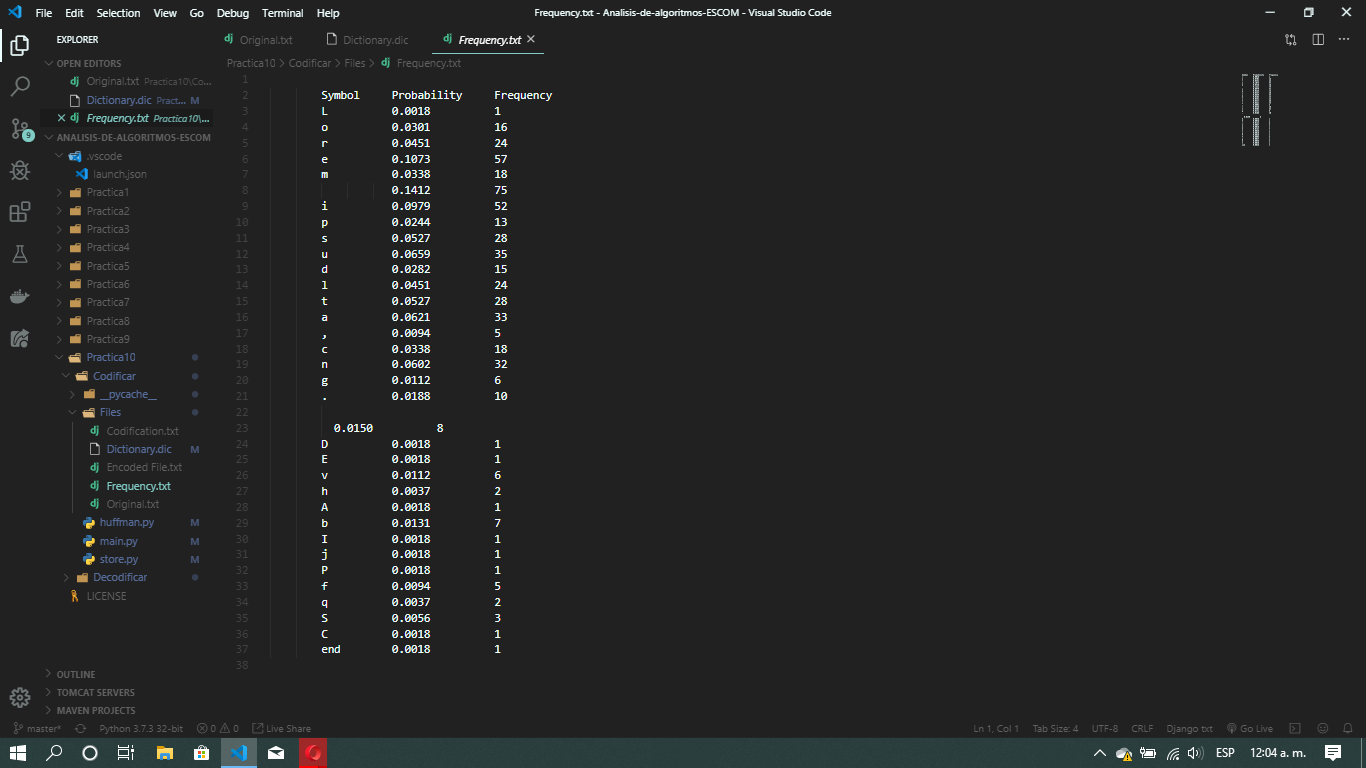
\includegraphics[width=10cm,keepaspectratio]{freq_huff.png}
    \caption{Diccionario de codificaci\'on y tabla de frecuencias.}
    \label{fig:huff_uno}
\end{figure}
\begin{figure}[ht]
    \centering
    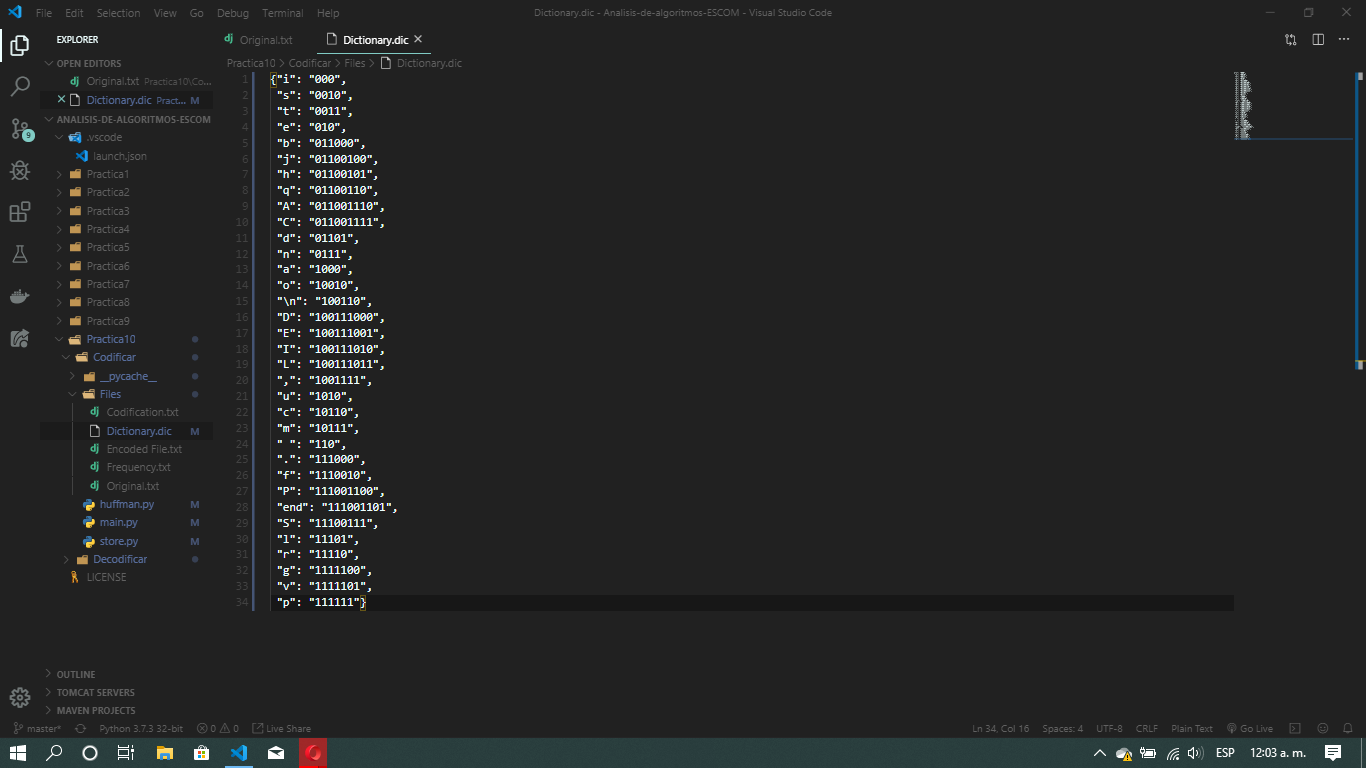
\includegraphics[width=10cm,keepaspectratio]{dicc_json_huff.png}
    \caption{Diccionario de codificaci\'on, en formato json.}
    \label{fig:huff_dos}
\end{figure}
\begin{figure}[ht]
    \centering
    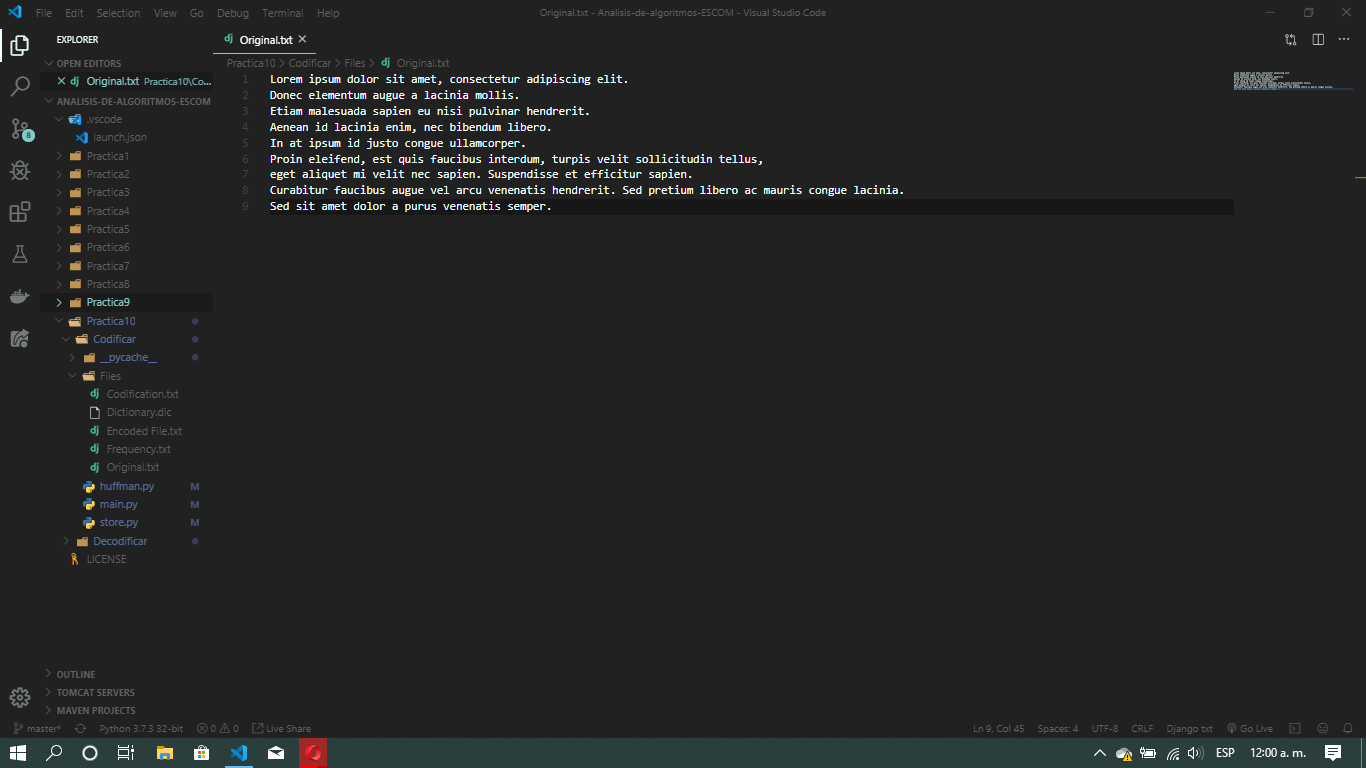
\includegraphics[width=10cm,keepaspectratio]{orig_huff.png}
    \caption{Archivo original usado como entrada}
    \label{fig:huff_tres}
\end{figure}
\begin{figure}[ht]
    \centering
    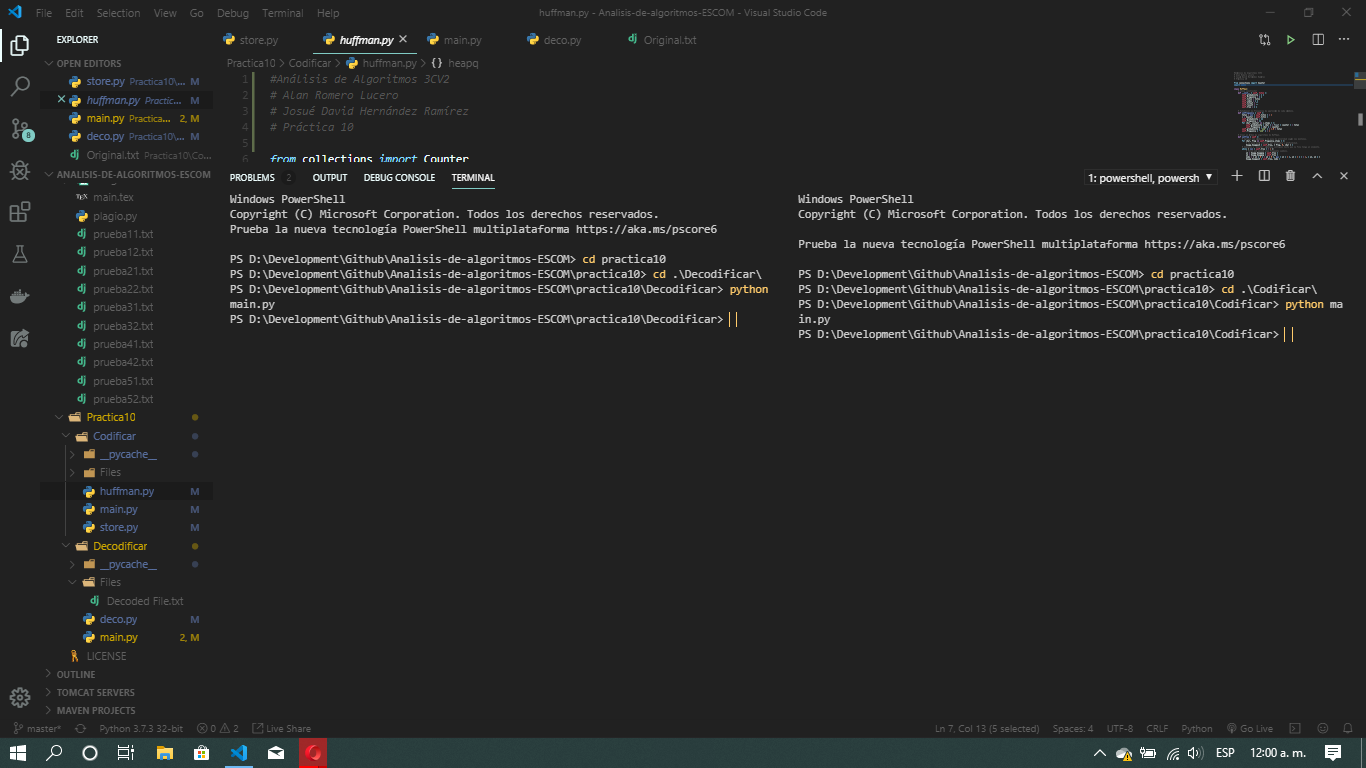
\includegraphics[width=10cm,keepaspectratio]{exec_huff.png}
    \caption{Ejecuci\'on del programa para codificaci\'on y decodificaci\'on}
    \label{fig:huff_cuatro}
\end{figure}

\begin{figure}[ht]
    \centering
    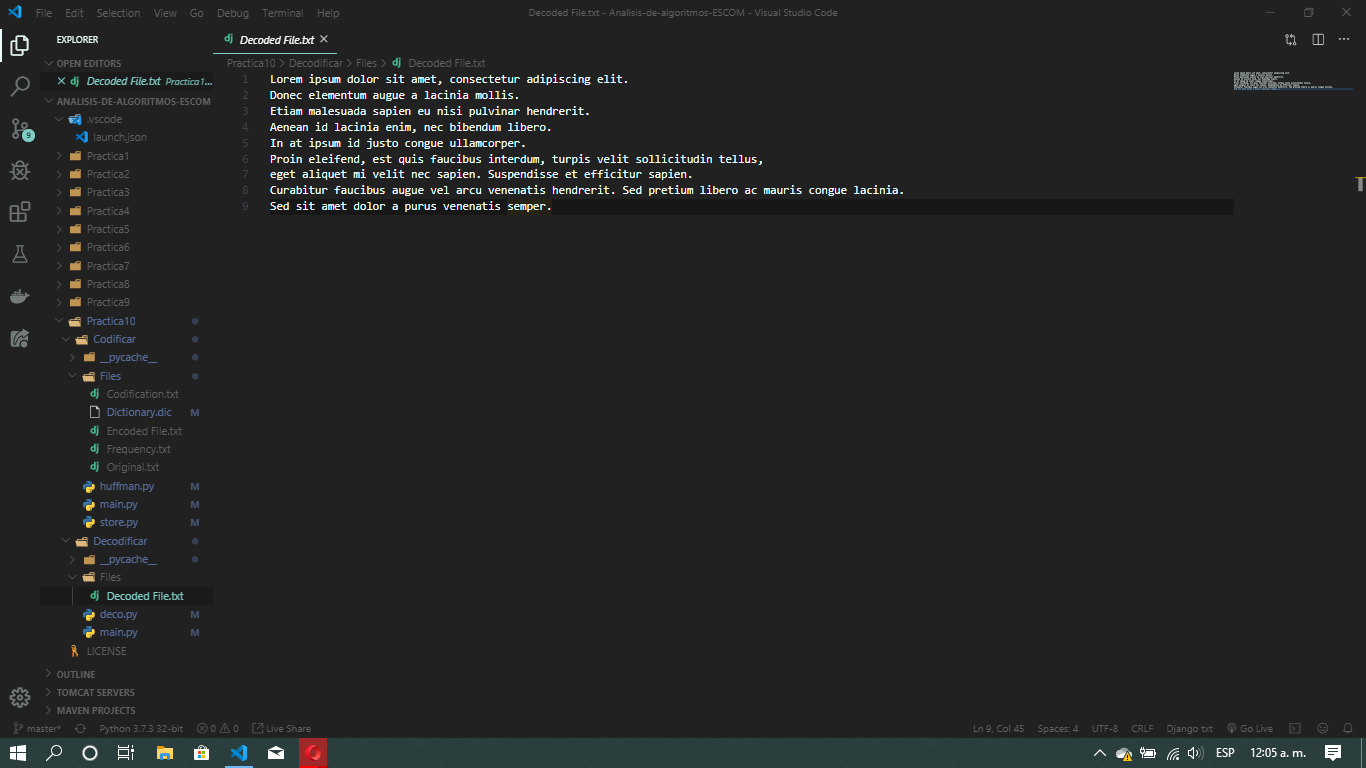
\includegraphics[width=10cm,keepaspectratio]{dec_huff.png}
    \caption{Archivo decodificado}
    \label{fig:huff_cinco}
\end{figure}

\begin{figure}[ht]
    \centering
    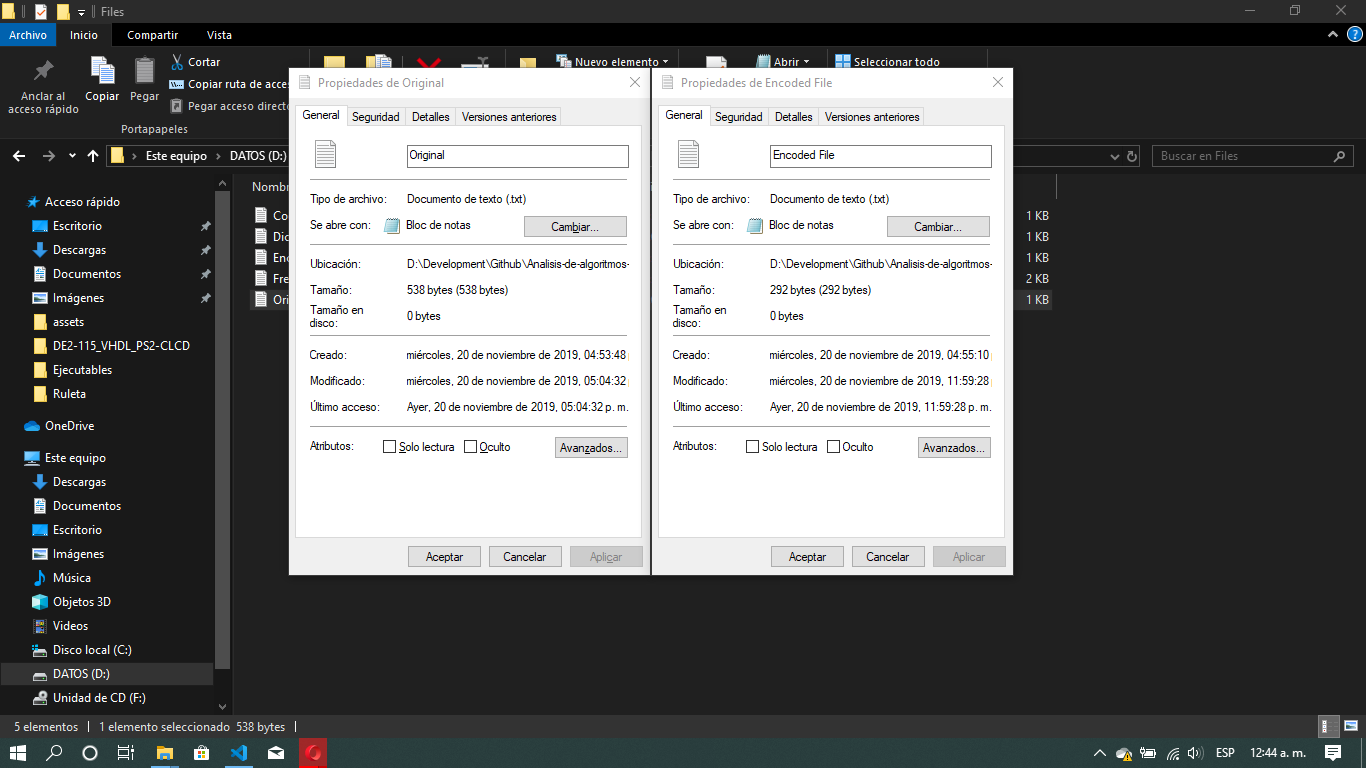
\includegraphics[width=10cm,keepaspectratio]{comp_huff.png}
    \caption{Comparaci\'on del tama\~no entre el archivo original y el archivo comprimido.}
    \label{fig:hufco}
\end{figure}

\newpage
\vfill
\clearpage

\section{Conclusiones}
\textit{Al\'an Romero Lucero}. La codificaci\'on Huffman me parece una manera muy inteligente de comprimir los archivos, as\'i como de aplicar conceptos tanto de probabilidad como de computaci\'on. Es interesante pensar como al crear este algoritmo de codificaci\'on se pens\'o en sustituir los car\'acteres m\'as repetidos con secuencias de bits m\'as cortas seg\'un la frecuencia con la que aparec\'ian en el texto.  Tambi\'en es interesante ver como se aplica una estrategia greedy, mediante los \'optimos locales de la codificaci\'on de cada car\'acter. Sin duda, un algoritmo interesante, que aunque es aparentemente simple el plantearlo de una manera tan brillante requiri\'o de un gran esfuerzo e ingenio.
\newline\newline
\textit{Josu\'e David Hern\'andez Ram\'irez}. 
Comprimir los archivos, antes era muy necesario puesto que los medios de almacenamiento de esa \'epoca ten\'ian muy poco espacio.
\newline
Para esto se bas\'o en los arboles binarios utilizando una fila de prioridad y con ese \'arbol de codificaci\'on se genera un diccionario, el cual va a ser utilizado para codificar el archivo. 
\newline
El uso de la probabilidad reduce bastante el peso del archivo como se puede observar en la figura \ref{fig:hufco} puesto que si reduce su peso considerablemente, esto haciendo pruebas \'unicamente con archivos de texto plano.
\newline
Es un algoritmo bastante interesante a tener en cuenta si se desea tener un poco de seguridad en archivos personales y ahorrar espacio en ciertos casos.


\section{Bibliograf\'ia}

[1] “Comprimiendo datos - el algoritmo de Huffman en Python,” Comprimiendo datos - el algoritmo de Huffman en Python – Bit y Byte – Explorando la intersección entre la ciencia de la computación y la ingeniería de software. [Online]. Available: http://bitybyte.github.io/Huffman-coding/. [Accessed: 20-Nov-2019]. 

\end{document}